\section{Sistemas de Información Geográfica}

Los Sistemas de Información Geográfica (GIS, por sus siglas en inglés) son sistemas que integran
software, hardware y datos para capturar, manejar, analizar y desplegar cualquier tipo de
información grográficamente referenciada.

GIS permite interactuar con la datos georeferenciados de manera gráfica, haciendo más entendible la
información de manera que se pueden revelar patrones, tendencias y relaciones en formas de mapas,
gráficos y reportes. 

Estos tipos de sistemas son relativamente nuevos, datan del año 1970 e inicialmente sólo estaban
disponibles para compañías y universidades que poseían un caro equipamiento computacional. Hoy en
día, cualquier persona que dispone de un computador puede utilizar GIS. De igual manera, los
Sistemas de Información Geográficos se han vuelto más fáciles de usar, existiendo aplicaciones que
pueden ser utilizadas por usuarios no especializados.

\subsection{Software GIS}
Normalmente son aplicaciones gráficas que pueden ser manipuladas usando mouse y teclado, aunque
existen otro tipo de software como librerías de desarrollo o extensiones para bases de datos.

Por lo general, las aplicaciones gráficas para GIS constan de cuatro componentes, como se ve en la
figura~\ref{aplicaciongis}: (1) un menú de aplicación, desde el cual se puede acceder a opciones
avanzadas o bien administración de archivos de la aplicación, (2) una barra de herramientas para
interactuar con el mapa, (3) un panel lateral donde se listan las capas de mapas y (4) la sección 
principal de la aplicación, que contiene el mapa.

\begin{figure}[h]
  \centering
  \caption{Estructura común de una aplicación GIS}
  \label{aplicaciongis}
  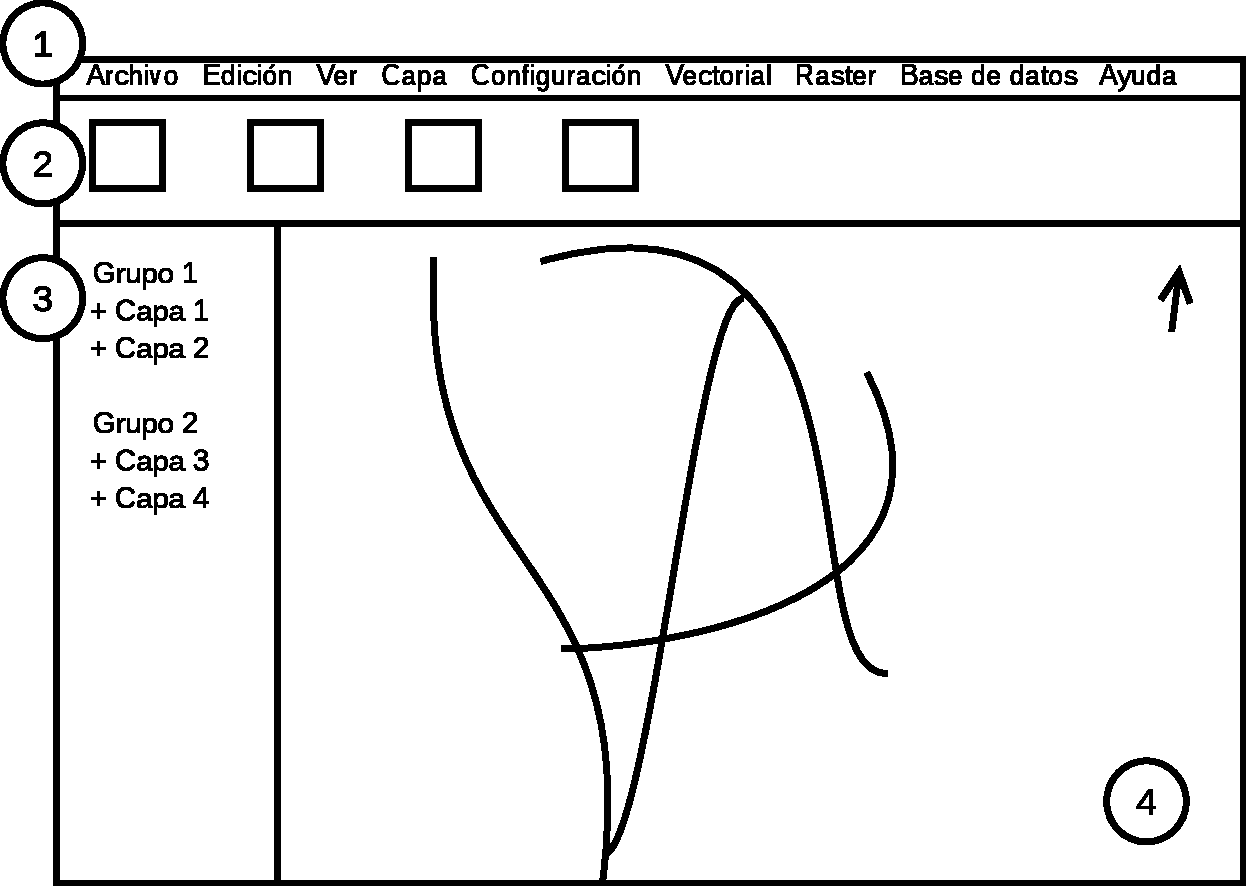
\includegraphics[scale=0.4]{gis_app}
\end{figure}

Este tipo de aplicaciones gráficas permite trabajar con capas, es decir, se pueden apilar distintos
mapas para obtener una visión completa, como podría ser el caso de un mapa que incluya la división
por predios de Valdivia superpuesto a un mapa que incluye la división por Unidades Vecinales de
Valdivia. El cruce visual de información es más simple de entender.

\subsection{Datos GIS}
Todos los datos que se trabajan en GIS son georeferenciados, es decir, contienen dentro de su
composición información relativa a su ubicación espacial. En el cuadro~\ref{datosgeo} se pueden
observar las filas de una tabla de una base de datos espacial en la que se almacenan puntos
específicos de un mapa.

\begin{table}[h]
  \centering
  \caption{Ejemplo de tabla con datos georeferenciados}
  \label{datosgeo}
  \begin{tabular}{|l|l|l|}
    \hline
    \textbf{Latitud} &  \textbf{Longitud}  & \textbf{Elemento} \\ \hline
    26.864239 & -35.898252 & Escombros \\
    34.221233 & -38.992713 & Paradero de micros \\
    26.921787 & -37.981889 & Bache \\
    \hline
  \end{tabular}
\end{table}

Los datos georeferenciados corresponden a la \emph{Latitud} y \emph{Longitud}. GIS permite mezclar
estos datos georeferenciados con otro tipo de información, como es el caso de la columna
\emph{Elemento}. Sin embargo, la potencialidad de GIS se descubre al hacer el cruce de información
entre elementos de bases de datos espaciales con otro tipo de bases de datos, como puede ser una
base de datos relacional que almacena información específica.

Los datos en GIS son almacenados en bases de datos espaciales, que tienen una estructura similar a
la mostrada en el cuadro~\ref{datosgeo}, esta base de datos espacial se puede definir de dos
maneras: (1) vectorial o (2) raster.

Los datos vectoriales son almacenados en pares de coordenadas X e Y dentro de la memoria del
computador. Los vectores son utilizados para representar puntos, líneas, polilíneas y áreas. Este
es el tipo de datos más utilizado y más flexible para su estudio y análisis. En la figura~\ref{mapa}
se pueden ver estos elementos marcados en un mapa vectorial.

\begin{figure}[h]
  \centering
  \caption{Ejemplo de mapa vectorial con áreas, polilíneas y puntos}
  \label{mapa}
  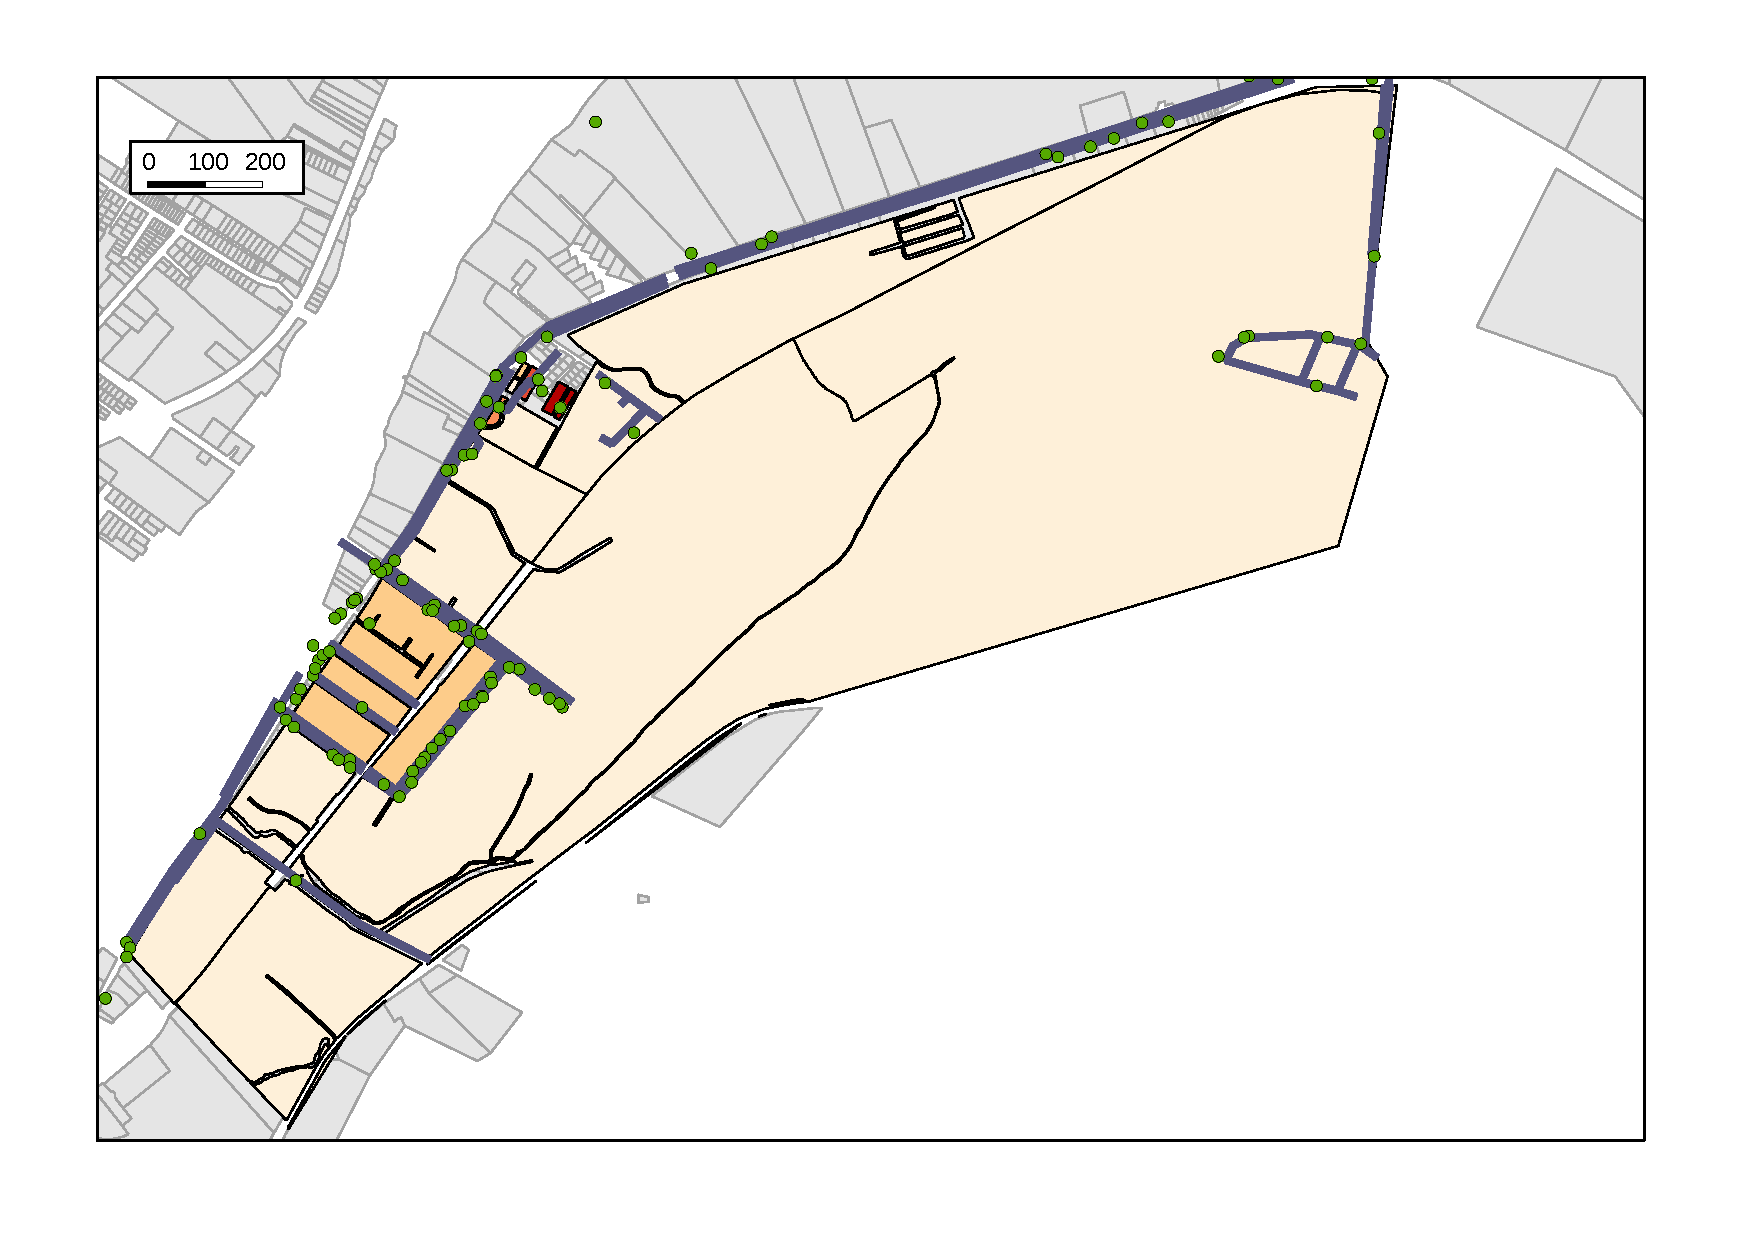
\includegraphics[scale=0.4]{mapa}
\end{figure}

Los datos de tipo raster son solo imágenes que incluyen un vector de referencia geográfica para
poder ubicarlo en las coordenadas del mapa. No son muy flexibles, pero sirven, por ejemplo, para
posicionar una capa con la imagen satelital de Valdivia y sobre ella ir trabajando con capas
vectoriales.

\subsection{Datos Vectoriales}

Los datos vectoriales permiten abstraer elementos del mundo real en una plataforma GIS, estos
elementos poseen atributos y son representados usando una geometría. Esta geometría es echa
interconectando uno o más vértices. Un vértice describe una posición en el espacio usando
coordenadas X, Y o, tal vez, Z. Las geometrías que incluyen un punto del eje Z son llamadas 2.5D, ya
que pueden describir la altura o la profundidad del vértice, pero no ambos.

Cuando un elemento geométrico está formado solo por un vértice, se denomina punto. Cuando consiste
en dos o más vértices se denomina polilínea. Cuando tiene cuatro o más vértices y el último vértice
es igual al primero, entonces se denomina polígono cerrado.

Cada uno de estos elementos incluye información adicional por sobre su geolocalización, a este tipo
de elementos se le llama base de datos espacial.

\subsection{Almacenamiento de Datos}
Existen dos mecanismos ampliamente utilizados para almacenar la información de los Sistemas de
Información Geográfico, cada uno con sus particularidades. La primera forma es a través de archivos,
como si se guardase un documento en algún software de procesamiento de palabras, por lo general se
utiliza el formato \emph{shape} de ESRI. Este formato
incluye tres tipos de archivos que corresponden a:
\begin{description}
  \item[Archivo ``.dbf'':] Archivo con los atributos de los elementos en la base de datos espacial
  \item[Archivo ``.shx''] Este archivo es un índice que ayuda a la aplicación GIS a encontrar
  elementos de manera más rápida.
  \item[Archivo ``.shp''] Archivo con la geometría de los elementos en la base de datos espacial.
\end{description}

Cuando se utiliza este mecanismo para guardar los datos se dispone de una manera rápida, fácil de
usar y descentralizada. Se deben entregar los tres archivos para que se pueda acceder a los datos.

La otra manera de almacenar los datos GIS es a través de bases de datos relacionales con extensiones
a bases de datos espaciales, tal es el caso de PostgreSQL con su extensión PostGIS, que permite a
este DBMS entender el tipo de datos geométrico donde se almacena la información de
georeferenciación. La ventaja de este método es que es increíblemente versátil para cruzar
información entre distintas tablas, que no todas tienen que ser espaciales, y permite crear nuevas
capas a partir de el cruce de datos, además, la centralización de la información hace que ésta se
mantenga estable, no fragmentada. Sin embargo, requiere de una conexión a la base de datos,
requiere de conocimientos básicos de SQL para poder hacer el cruce de datos.
